\documentclass[12pt, a4paper, oneside]{ctexart}
\usepackage{amsmath, amsthm, amssymb, bm, color, framed, graphicx, hyperref, mathrsfs, mathtools, enumerate, tikz}
\usepackage{float}
\usepackage{subcaption} 



\usetikzlibrary{patterns}

\title{\textbf{Homework 7}}
\author{萃英学院\qquad 2022级\qquad 王一鑫}
\date{\today}
\linespread{1.5}
\newcounter{problemname}
\newenvironment{problem}{\begin{framed}\stepcounter{problemname}\par\noindent\textsc{Problem \arabic{problemname}. }}{\end{framed}\par}
\newenvironment{solution}{%
	\par\noindent\textsc{Solution. }\ignorespaces
}{%
	\hfill$\qed$\par
}
\newenvironment{note}{\par\noindent\textsc{Note of Problem \arabic{problemname}. }}{\\\par}

\begin{document}
	
	\maketitle
	
	\begin{problem}
		(Exercise 4.5)

        (i) For which values of \( k \) is the \( k \)-cube \( Q_k \) planar?

        (ii) For which values of \( r \), \( s \), and \( t \) is the complete tripartite graph \( K_{r,s,t} \) planar?


	\end{problem}
    
	\begin{solution}
        \begin{enumerate}[(i)]
            \item $k\geq3$. This is because when $k = 4$, $Q_k$ contains $K_{3,3}$. Moreover, 
            $Q_{k}$ can be constructed by two $Q_{k-1}$, so $Q_{k}$ is not planar ($k\geq4$).
            \item Without loss of generality assume \( r \geq s \geq t \).

            If \( r \geq 3 \), and \( s + t \geq 3 \), then the graph is not planar (It contains $K_{3,3}$).
            
            In the cases \( r \leq 2 \) or \( s + t \leq 2 \), it is planar.
            
        \end{enumerate}
	    
		
	\end{solution}
		

		
	
	\begin{problem}
		(Exercise 4.7)

        Prove that the Petersen graph is non-planar

        (i) by removing the two 'horizontal' edges and using Theorem 4.2;

        (ii) by using Theorem 4.3.


	\end{problem}
	
	\begin{solution}
		\begin{enumerate}[(i)]
            
            \item By removing the two 'horizontal' edges we find that Petersen graph contains $K_{3,3}$, shown in Fig \ref{fig:K33}.
            \begin{figure}[H]
                \small
                \centering
                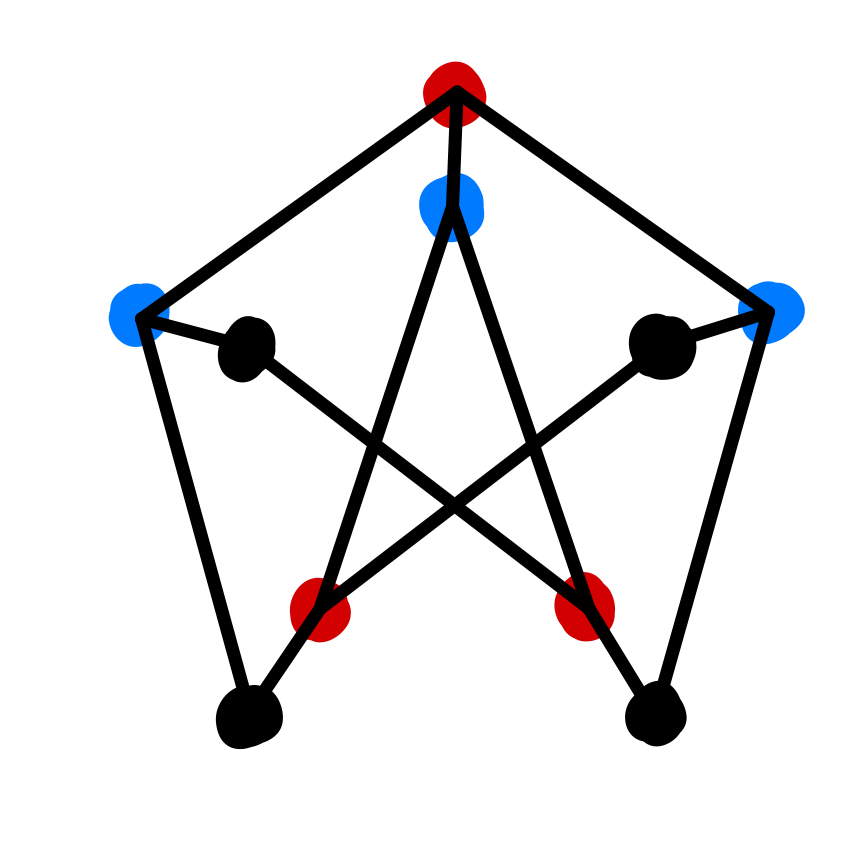
\includegraphics[width=0.32\columnwidth]{figure/fig1.jpg}
                \caption{$K_{3,3}$}
                \label{fig:K33}
            \end{figure}
            By Theorem 4.2, Petersen graph is not planar.
            \item Petersen graph is contractible to $K_5$ as Fig \ref{fig:K5}. Apply Theorem 4.3.
            \begin{figure}[H]
                \small
                \centering
                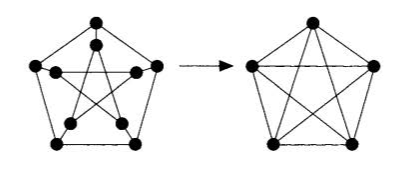
\includegraphics[width=0.75\columnwidth]{figure/fig2.png}
                \caption{$K_{5}$}
                \label{fig:K5}
            \end{figure}
        \end{enumerate}
		
	\end{solution}
	
	\begin{problem}
        (Exercise 4.9)

        If two homeomorphic graphs have \( n_i \) vertices and \( m_i \) edges (\( i = 1, 2 \)), show that

        \[
        m_1 - n_1 = m_2 - n_2.
        \]


	\end{problem}
	
	\begin{solution}
       
        Any graph is homeomorphic to a graph with no vertices of degree 2. 
        In the process of removing a vertex of degree 2, we will lose one vertex and one edge, 
        so the difference $m - n$ is unchanged. Therefore, it suffices to show that 
        homeomorphic graphs with no vertices of degree 2 are isomorphic 
        (and so have the same number of vertices and the same number of edges). 
        This is because, in the absence of vertices of degree 2, a homeomorphism 
        between two graphs must take vertices to vertices and edges to edges.

        
	\end{solution}
	
	
	
	\begin{problem}
        (Exercise 4.10) 
        
        A planar graph \( G \) is outerplanar if \( G \) can be drawn in the plane so that all of its vertices lie on the exterior boundary.

        (i) Show that \( K_4 \) and \( K_{2,3} \) are not outerplanar.

        (ii) Deduce that, if \( G \) is an outerplanar graph, then \( G \) contains no subgraph homeomorphic or contractible to \( K_4 \) or \( K_{2,3} \).

        (The converse result also holds, yielding a Kuratowski-type criterion for a graph to be outerplanar.)

		
	\end{problem}
	
	\begin{solution}
        
        \begin{enumerate}[(i)]
            \item Let $G'$ be obtained from $G$ by adding an extra vertex to $G$ adjacent to every other 
        vertex. Then $G'$ is planar if and only if $G$ is outerplanar. By Theorem 4.1 we know that 
        $K_5$ and $K_{3,3}$ are non-planar, thus \( K_4 \) and \( K_{2,3} \) are not outerplanar.
            \item Kuratowski's theorem shows that if \( G' \) is planar, then \( G' \) 
            contains no subgraph homeomorphic or contractible to \( K_5 \) or \( K_{3,3} \).By the
            argument in (i), \( G \) contains no subgraph homeomorphic or contractible to \( K_4 \) or \( K_{2,3} \).
            
        \end{enumerate}

		
	\end{solution}


	\begin{problem}
		(Exercise 4.11)

        By placing its vertices at the points
        \((1, 1^2, 1^3) \), \((2, 2^2, 2^3)\), \((3, 3^2, 3^3)\), $\cdots$, 
        prove that any simple graph can be drawn without crossings in Euclidean three-dimensional 
        space so that each edge is represented by a straight line.

		
    \end{problem}

	\begin{solution}
       
    If there are two crossing edges with endpoints on that curve, then the endpoints 
    are four coplanar points on the curve. Call the points 
    $(t_i, t_i^2, t_i^3)$, $i = 1, 2, 3, 4$, where $t_1, t_2, t_3, t_4$ 
    are distinct real numbers, and suppose they all lie on a plane $A + Bx + Cy + Dz = 0$ 
    where $A, B, C, D$ are not all zero. Then $A, B, C, D$ satisfy the equation

    \[
    \begin{bmatrix}
    1 & t_1 & t_1^2 & t_1^3 \\
    1 & t_2 & t_2^2 & t_2^3 \\
    1 & t_3 & t_3^2 & t_3^3 \\
    1 & t_4 & t_4^2 & t_4^3
    \end{bmatrix}
    \begin{bmatrix}
    A \\
    B \\
    C \\
    D
    \end{bmatrix}
    =
    \begin{bmatrix}
    0 \\
    0 \\
    0 \\
    0
    \end{bmatrix}
   \]

    However, since the coefficient matrix is a nonsingular Vandermonde matrix, 
    the equation has no nontrivial solution.
    Thus any simple graph can be drawn without crossings in Euclidean three-dimensional 
    space so that each edge is represented by a straight line.


    \end{solution}
		
    
	\begin{problem}
		(Exercise 4.15)

    \begin{enumerate}
        \item[(i)] Use Euler's formula to prove that, if $G$ is a connected planar graph of 
        girth 5 with $n$ vertices and $m$ edges, then $m \leq \frac{5}{3}(n - 2)$. 
        Deduce that the Petersen graph is non-planar.
        
        \item[(ii)] Obtain an inequality, generalizing that in part (i), for connected planar 
        graphs of girth $r$.
    \end{enumerate}

    \end{problem}

	\begin{solution}
		\begin{enumerate}[(i)]
            \item 	Since $G$ has girth 5, we have $5f \leq 2m$. 
            Combining this with Euler's formula $n - m + f = 2$ gives the required inequality. 
            \[ 5(2-n+m) \leq 2m \Leftrightarrow m\leq \dfrac{5}{3}(n-2)\]
            If the Petersen graph were planar, then this inequality would be 
            $15 \leq \dfrac{40}{3}$, which is false. Thus, the Petersen graph is non-planar.
            \item   If $G$ has girth $r$, then $rf \leq 2m$. 
            Combining this with Euler's formula gives the inequality
            \[
            r(2-n+m) \leq 2m \Leftrightarrow m \leq \frac{r(n - 2)}{r - 2}.
            \]

        \end{enumerate}

       

		
	\end{solution}


	\begin{problem}
		(Exercise 4.16)
        
        Let $G$ be a polyhedron (or polyhedral graph), each of whose faces is bounded by a pentagon or a hexagon.
        \begin{enumerate}
            \item[(i)] Use Euler's formula to show that $G$ must have at least 12 pentagonal faces.
            \item[(ii)] Prove, in addition, that if $G$ is such a polyhedron with exactly three faces meeting at each vertex (such as a football), then $G$ has exactly 12 pentagonal faces.
        \end{enumerate}
        

	\end{problem}

	\begin{solution}
        \begin{enumerate}[(i)]
            \item By the property of polyhedron, we have $n \leq \frac{2}{3} m$, 
            so that $-n \geq -\frac{2}{3} m$ and so, by Euler's formula, we have:

            \[
            f = 2 + m - n \geq 2 + m - \frac{2}{3} m = 2 + \frac{1}{3} m.
            \]
            Now if we have have $p$ pentagonal faces and $h$ hexagonal faces, 
            then there are $p + h$ faces, so $p + h = f$. and $5p + 6h = 2m$ 
            \[p+h\geq 2 + \dfrac{1}{6}(5p + 6 h) \Leftrightarrow p\geq 12\]
            \item Now $v = \frac{2}{3} e$, we can change the inequality to equality.

        \end{enumerate}
    
	\end{solution}
     

    \begin{problem}
        (Exercise 4.17)

        Let $G$ be a simple plane graph with fewer than 12 faces, in which each vertex has degree at least 3.
        \begin{enumerate}
            \item[(i)] Use Euler's formula to prove that $G$ has a face bounded by at most four edges.
            \item[(ii)] Give an example to show that the result of part (i) is false if $G$ has 12 faces.
        \end{enumerate}


       
    \end{problem}
	
    \begin{solution}
       \begin{enumerate}[(i)]
        \item By problem 7 we have 
            \[
            f  \geq = 2 + \frac{1}{3} m.
            \]
        If not, then $G$ has faces bounded by at least $5$ edges, that is $5f \leq 2m$.
        \[10 + \frac{5}{3}m\leq 2 m\Rightarrow m \geq 30\]
        Thus, $f \geq 2 + \frac{1}{3} m \geq 12$, which is a contradiction since
        $G$ is a simple plane graph with fewer than $12$ faces.
        \item The situation in Problem 7 (ii).
       \end{enumerate} 
        
    \end{solution}

    \begin{problem}
        (Exercise 4.18)

        \begin{enumerate}
            \item[(i)] Let $G$ be a simple connected cubic plane graph, and let $C_k$ be the number of $k$-sided faces. By counting the number of vertices and edges of $G$, prove that
            \[
            3C_3 + 2C_4 + C_5 - C_7 - 2C_8 - 3C_9 - \cdots = 12.
            \]
            \item[(ii)] Use this result to deduce the result of Exercise 4.16(ii).
            \item[(iii)] Deduce also that $G$ has at least one face bounded by at most five edges.
        \end{enumerate}

    \end{problem}

    \begin{solution}
        \begin{enumerate}
            \item[(i)] If $G$ has $n$ vertices, $m$ edges, and $f$ faces, then
            \begin{align*}
                f &= C_3 + C_4 + C_5 + C_6 + \dots, \\
                2m &= 3C_3 + 4C_4 + 5C_5 + 6C_6 + \dots, \\
                3n &= 3C_3 + 4C_4 + 5C_5 + 6C_6 + \dots.
            \end{align*}
            The last equality is from the definition of cubic graph.
            Substituting these expressions for $f$, $m$, and $n$ into Euler's formula yields the result.
        
            \item[(ii)] Since $C_3 = C_4 = C_7 = C_8 = \dots = 0$, we deduce that $C_5 = 12$.
        
            \item[(iii)] If $G$ has no face bounded by at most five edges, then $C_3 = C_4 = C_5 = 0$, and the left-hand side is negative; this is a contradiction.
        \end{enumerate}
        
    \end{solution}
\end{document}


